\chapter{\textit{Frameworks} MVC e de Persistência}\label{cap:frameworksPersistencia}
\epigraph{``\textit{A persistência é o caminho do êxito}''.}{Charles Chaplin}

\lettrine[lines=4, lhang=0.1, lraise=0, loversize=0.2, findent=0.1em]{\textcolor{corTema}{N}}{ESTE} Capítulo reconstruiremos o ``Sistema de Venda de Produtos'' do Capítulo~\ref{cap:sistemaVendaProdutos} utilizando diversos \textit{frameworks} que tornarão nosso trabalho menos tedioso e mais direto ao ponto! A partir de agora não construiremos os nossos exemplos em sua completude, pois focaremos nas novidades e não queremos Capítulos muito extensos. Os projetos prontos estarão disponíveis como nos Capítulos anteriores.

\vfill

\section{Introdução}

Antes de começarmos a trabalhar, precisamos configurar nosso ambiente de desenvolvimento. Como lidaremos com grande parte da \textit{stack} de \textit{frameworks} e bibliotecas do Spring, poderíamos utilizar a ferramenta oficial deles para nos auxiliar, a Spring Tool Suite 4, mas não faremos isso. Eu particularmente não sou muito fã, pois ela é baseada na IDE Eclipse que, na minha opinião, é extremamente burocrática e instável, mas como ela é adotada como o padrão da indústria, uma hora ou outra acabamos ter que a adotar. Continuaremos a utilizar o NetBeans como nossa ferramenta padrão, mas você pode testar a Spring Tool Suite caso deseje. No momento em que este texto está sendo escrito, existem também versões para o Visual Studio Code (\url{https://code.visualstudio.com/}) a para a IDE Theia (\url{https://theia-ide.org/}). O \textit{download} de qualquer uma das versões pode ser feito em \url{https://spring.io/tools}.


\subsection{Criando a Primeira Aplicação Spring Boot}

A primeira coisa que vamos fazer é acessar o site Spring Initializr (\url{https://start.spring.io/}). Nesse site podermos configurar a infraestrutura básica do nosso projeto, que utilizará o Maven (\url{https://maven.apache.org/}) como ferrameta de gerenciamento do projeto. O Maven é suportado atualmente pelas principais IDEs disponíveis. Sendo um projeto Maven, espera-se que todas as IDEs trabalhem de forma semelhante, então teoriacemente podemos trabalhar com mais de uma ferramenta no mesmo projeto. Note que iremos reconstruir o ``Sistema de Venda de Produtos'' do Capítulo\ref{cap:sistemaVendaProdutos}. Vamos começar?

A versão atual da página principal do site do Spring Initializr pode ser vista na Figura~\ref{fig:cap10SpringInitializr}.

\FloatBarrier
\begin{figure}[!htbp]
    \centering
    \caption{Tela principal do site do Spring Initializr}
    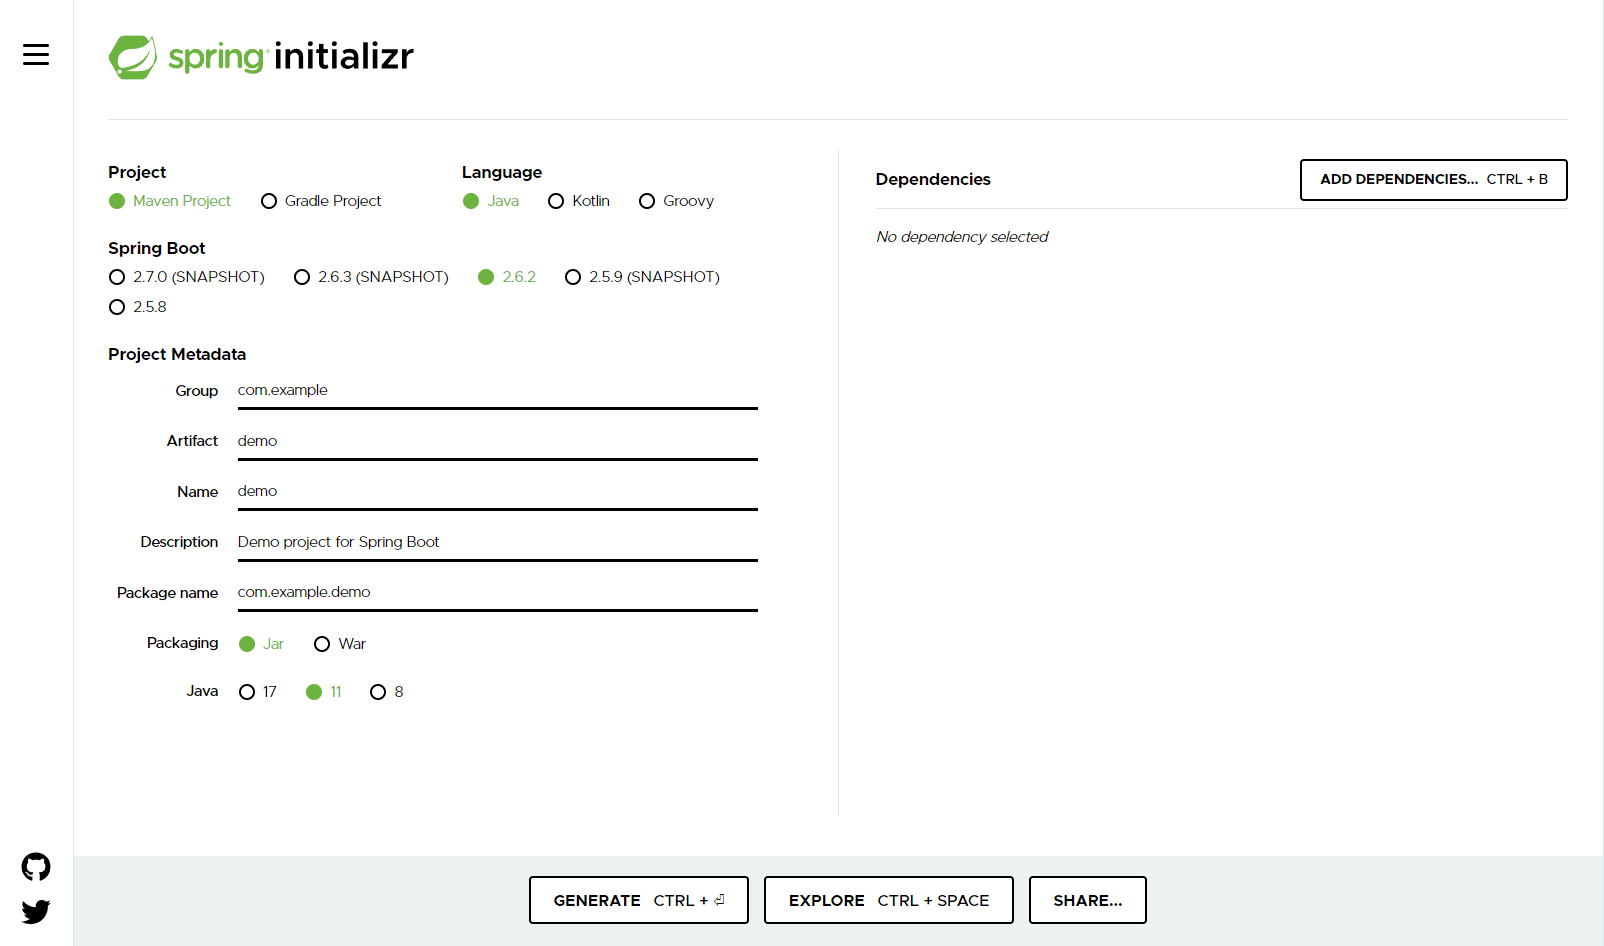
\includegraphics[scale=0.4]{imagens/cap10SpringInitializr}
    \\\textbf{Fonte:} \url{https://start.spring.io/}
    \label{fig:cap10SpringInitializr}
\end{figure}
\FloatBarrier

Basicamente, do lado esquerdo temos as opções de configuração do projeto:

\begin{itemize}

    \item \textbf{\textit{Project}:} qual ferramenta de gerencimanto de projetos que será usada (usaremos o Maven);
    
    \item \textbf{\textit{Language}:} a linguagem de programação utilizada no projeto;
    
    \item \textbf{\textit{Spring Boot}:} qual a versão do Spring Boot que usaremos;
    
    \item \textbf{\textit{Project Metadata}:} os metadados do projeto, que envolvem:
    
    \begin{itemize}
    
        \item \textbf{\textit{Group}:} nome do identificador do grupo do projeto, normalmente igual ao pacote da organização/empresa do desenvolvedor do projeto, seguindo as regras para nomeação de pacotes da linguagem Java (\url{https://docs.oracle.com/javase/specs/jls/se6/html/packages.html#7.7});
        
        \item \textbf{\textit{Artifact}:} nome do arquivo que será gerado (sem a extensão \texttt{.jar} ou \texttt{.war}) após a construção do projeto e também o identificador que será usado pelo Maven para encontrar a versão compilada e instalada do projeto dentro de seu repositório local. Normalmente se o identificador do artefato tiver mais de uma palavra, separamos as mesmas por hífens;
        
        \item \textbf{\textit{Name}:} nome do projeto, o que aparecerá na raiz do projeto aberto nas IDEs para identificá-los;
        
        \item \textbf{\textit{Description}:} breve descrição do projeto;
        
        \item \textbf{\textit{Project name}:} pacote raiz do projeto, usando como prefixo o identificador do grupo. Caso sejam usados hífens~\footnote{O Spring Initializr usará automaticamente o valor do identificador artefato aqui, trazendo hífens, que serão descartados no pacote final}, eles serão suprimidos no projeto gerado;
        
        \item \textbf{\textit{Packaging}:} tipo de empacotamento que será feito. Arquivos \texttt{.jar} podem ser executados localmente e arquivos \texttt{.war} são destinados à implantação em servidores de aplicações e/ou contêineres de Servetls. A geração de pacotes \texttt{.war} será ensinada mais adiante neste Capítulo;
        
        \item \textbf{\textit{Java}:} a versão do Java que se quer usar. Note que apenas as versões \textit{Long-Term Support} (LTS) aparecem e, além disso, você precisa ficar atento para ter um JDK de versão igual ou superior instalado na máquina de desenvolvimento e na máquina em que o projeto for executar em produção.
        
    \end{itemize}
\end{itemize}

Sabendo disso, vamos agora preparar o nosso projeto de acordo com o apresentado na Figura~\ref{fig:cap10SpringInitializrConfProjeto01}:

\FloatBarrier
\begin{figure}[!htbp]
    \centering
    \caption{Definição das propriedades do projeto}
    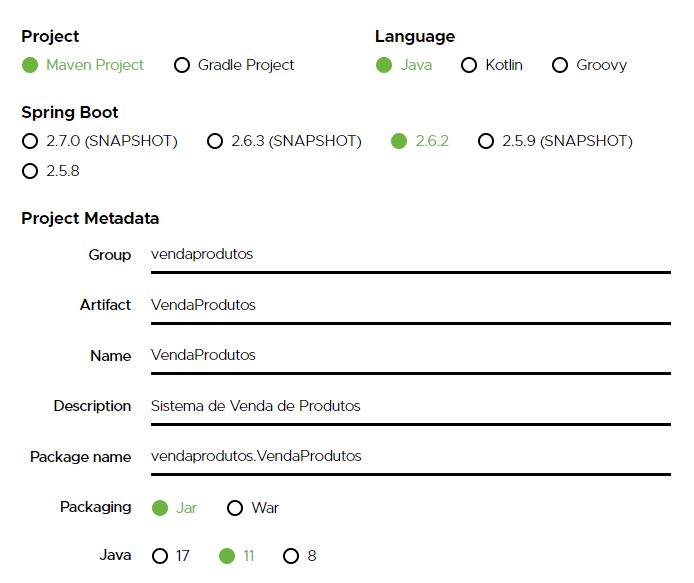
\includegraphics[scale=0.7]{imagens/cap10SpringInitializrConfProjeto01}
    \\\textbf{Fonte:} \url{https://start.spring.io/}
    \label{fig:cap10SpringInitializrConfProjeto01}
\end{figure}
\FloatBarrier

Ou seja:

\begin{itemize}

    \item \textbf{\textit{Project}:} usaremos o Maven;
    
    \item \textbf{\textit{Language}:} programaremos em Java;
    
    \item \textbf{\textit{Spring Boot}:} a última versão estável do Spring Boot, nesse caso, a 2.6.2. Note que isso pode variar de acordo com a época que você estiver lendo esse texto;
    
    \item \textbf{\textit{Project Metadata}:} os metadados do projeto, que envolvem:
    
    \begin{itemize}
    
        \item \textbf{\textit{Group}:} usaremos \texttt{dsoc7}, que é a sigla da disciplina do curso de Bacharelado em Ciência da Computação do Instituto Federal de Educação, Ciência e Tecnologia de São Paulo\footnote{Câmpus São João da Boa Vista}, para a qual esse livro foi desenvolvido incialmente, mas em um caso real, você deve preencher com a notação de domínio inverso da empresa ou instituição para a qual estiver desenvolvendo o projeto. Por exemplo, se a instuição tem o domínio \texttt{ifsp.edu.br}, você deverá preencher o identificador do grupo com \texttt{br.edu.ifsp}. Caso seja um projeto pessoal e você possuir um domínio, a regra é a mesma. Eu por exemplo tenho o domínio \texttt{davidbuzatto.com.br}, então meu identificador de grupo, para um projeto pessoal, deveria ser \texttt{br.com.davidbuzatto};
        
        \item \textbf{\textit{Artifact}:} usaremos \texttt{venda-produtos-spring};
        
        \item \textbf{\textit{Name}:} o nome preencheremos com \texttt{VendaProdutosSpring}, que é o que aparecerá no NetBeans na raiz do projeto. Aqui em um caso real você poderia usar espaços para nomear o projeto. Eu prefiro sem espaços. Note que para diferenciar do primeiro projeto de venda de produtos, adicionaremos o sufixo Spring;
        
        \item \textbf{\textit{Description}:} preencher com Sistema de Venda de Produtos Usando Spring Boot;
        
        \item \textbf{\textit{Project name}:} aqui o Spring Initializr já deve ter preenchido com a concatenção do identificador do grupo e do identificador do artefato, ficando \texttt{dsoc7.venda-produtos-spring}. Na criação do projeto esses hífens serão retirados, pois nomes de pacotes em Java não podem ter hífem;
        
        \item \textbf{\textit{Packaging}:} usaremos empacotamento em \texttt{.jar}, que é o padrão mesmo que não seja informado;
        
        \item \textbf{\textit{Java}:} usaremos o Java 11.
        
    \end{itemize}
\end{itemize}

Com isso feito, temos a configuração básica do projeto pronta, mas ainda precisamos adicionar as primeiras dependências que utilizaremos. As dependências são basicamente as bibliotecas que usaremos no projeto. A vantagem de usar um sistema de gerenciamento de projetos como o Maven é que, ao adicionarmos dependências no projeto, ele se encarregará de carregar todas as dependências que uma dependência depende, inclusive com as versões apropriadas! Nossa vida fica muito mais fácil, sem precisarmos ficar lidando com a definição de bibliotecas e isso é um super avanço na produtividade!

Para adicionar uma dependência, clique no botão \destaque{\textit{ADD DEPENDENCIES...}}. Ao fazer isso, um diálogo aparecerá, onde você poderá escolher as dependências do projeto. Ao encontrar a dependência desejada, basta clicar nela que ela será inserida na lista de dependências do projeto. Você pode procurar pelas dependências rolando a lista ou então pesquisando na caixa de texto acima. No nosso projeto utilizaremos sete dependências, apresentadas na Figura~\ref{fig:cap10SpringInitializrConfProjeto02} e descritas a seguir.

\FloatBarrier
\begin{figure}[!htbp]
    \centering
    \caption{Definição das dependências do projeto}
    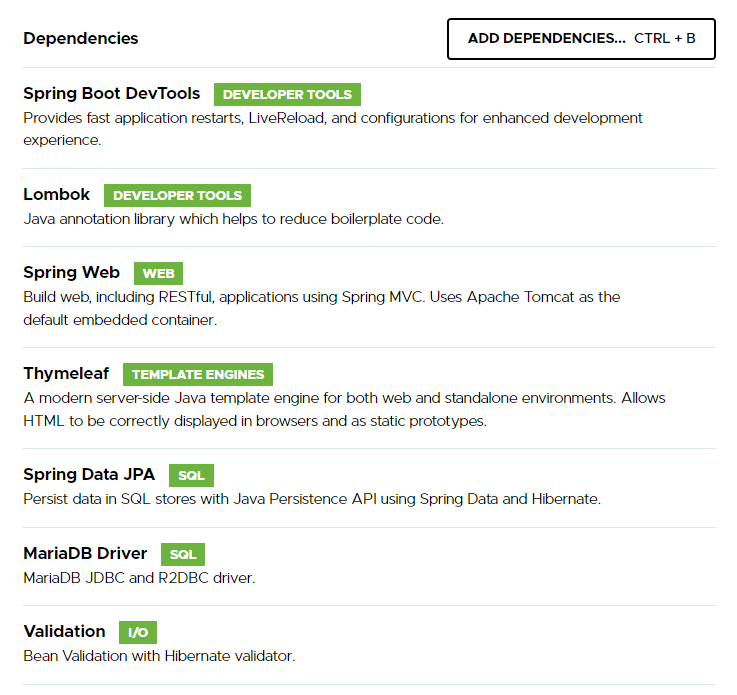
\includegraphics[scale=0.7]{imagens/cap10SpringInitializrConfProjeto02}
    \\\textbf{Fonte:} \url{https://start.spring.io/}
    \label{fig:cap10SpringInitializrConfProjeto02}
\end{figure}
\FloatBarrier

\begin{itemize}

    \item \textbf{Spring Boot DevTools:} auxília no desenvolvimento de aplicações usando Spring Boot, permitindo reinicialização rápida do servidor embarcado, integração com LiveReload etc;
    
    \item \textbf{Lombok:} é uma biblioteca de anotações que nos ajuda na criação automática de código padronizado como getters, setters, construtores etc;
    
    \item \textbf{Spring Web:} apoia a construção de aplicações Web usando o padrão de projeto MVC através do \textit{framework} Spring MVC, além da criação de Web Services RESTful;
    
    \item \textbf{Thymeleaf:} é uma \textit{template engine} que permite a definição de modelos para a criação de interfaces gráficas usando HTML, diminuindo a duplicidade de código e facilitando a manutenção;
    
    \item \textbf{Spring Data JPA:} \textit{framework} para persistência de dados usando Hibernate e a Java Persistence API (JPA);
    
    \item \textbf{MariaDB Driver:} driver de conexão com MariaDB, o SGBD que estamos utilizando neste livro;
    
    \item \textbf{Validation:} permite a validação de objetos de dados\footnote{Esses objetos são aqueles que estamos criando a partir das classes de modelo. Podemos chamá-los também de \textit{Data Transfer Objects} (DTO)} que serão gerenciados pela aplicação. Essa validação já foi feita automaticamente nos últimos projetos, você se lembra?
    
\end{itemize}

Agora com o inicializador do projeto configurado, clique no botão \destaque{\textit{GENERATE}}. Ao fazer isso, um arquivo \texttt{.zip} será baixado, com o nome de \texttt{venda-produtos-spring.zip}. No local onde foi salvo, descompacte-o. Abra o NetBeans e realize o procedimento de abrir projetos. Vá à pasta onde o arquivo foi descompactado. Você notará que o NetBeans reconhecerá um projeto Maven ali. Selecione-o e abra-o.

As configurações iniciais do projeto gerado no Spring Initilizr podem ser compartilhadas. Sendo assim, se você quiser, pode usar o \textit{link} abaixo para fazer o \textit{download} do projeto com as mesmas configurações apresentadas.

\url{https://start.spring.io/#!type=maven-project&language=java&platformVersion=2.6.2&packaging=jar&jvmVersion=11&groupId=dsoc7&artifactId=venda-produtos-spring&name=VendaProdutosSpring&description=Sistema%20de%20Venda%20de%20Produtos%20Usando%20Spring%20Boot&packageName=dsoc7.venda-produtos-spring&dependencies=devtools,lombok,web,thymeleaf,data-jpa,mariadb,validation}

Provavelmente, após abrir o projeto, seu NetBeans vai demorar alguns minutos --pode demorar bastante na verdade-- para baixar o índice do repositório central do Maven e prepará-lo no seu computador. Após esse processo, seu NetBeans vai ``reclamar'', informando que o repositório do Maven local não tem uma cópia das dependências do projeto. Veja na Figura~\ref{fig:cap10ConfProjeto03} o que provavelmente aparecerá, ou seja, um sinal de aviso (\textit{warning}) no ícone do projeto.

\FloatBarrier
\begin{figure}[!htbp]
    \centering
    \caption{Resolução de problema do projeto criado}
    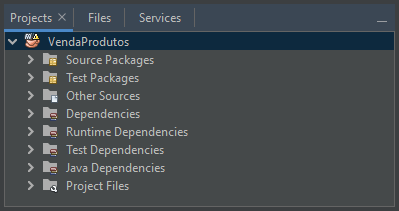
\includegraphics[scale=1]{imagens/cap10ConfProjeto03}
    \\\textbf{Fonte:} Elaborada pelo autor
    \label{fig:cap10ConfProjeto03}
\end{figure}
\FloatBarrier

Para resolvermos isso, faremos algo que talvez você já tenha feito para outras situações. Clique com o botão direito no projeto e escolha a opção \destaque{\textit{Resolve Project Problems...}} do menu de contexto. Fazendo isso, um diálogo aparecerá com um ou mais itens com o texto ``\textit{Some dependency artifacts are not in the local repository}'', indicando o problema encontrado. Clique no botão \destaque{\textit{``Resolve''}}. O Maven vai começar a realizar o processo de ``\textit{Priming}'' (preparação) do projeto, prepararando e baixando todas as dependências. Essa preparação pode demorar um pouco também. Você saberá que o processo terminou quando aparecer ``BUILD SUCESS'' na saída do NetBeans e quando o diálogo da solução dos problemas do projeto apresentar o problema apontado anteriormente com um ``check'' ou ``tick'' verde. Após esse processo, clique em \destaque{\textit{Close}}.

Agora que criamos o projeto no Spring Initializr e o abrimos no NetBeans, vamos entender sua estrutura, a qual é mostrada com seus principais nós expandidos na Figura~\ref{fig:cap10EstruturaProjeto}

\FloatBarrier
\begin{figure}[!htbp]
    \centering
    \caption{Estrutura do projeto}
    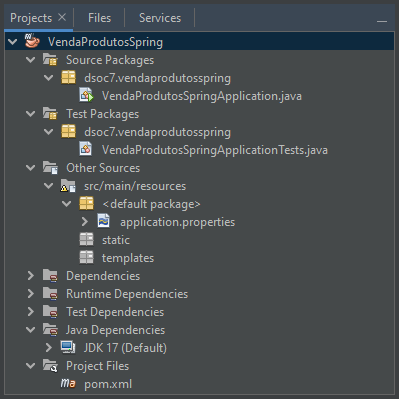
\includegraphics[scale=1]{imagens/cap10EstruturaProjeto}
    \\\textbf{Fonte:} Elaborada pelo autor
    \label{fig:cap10EstruturaProjeto}
\end{figure}
\FloatBarrier

As pastas \destaque{\textit{Source Packages}} e \destaque{\textit{Test Packages}} servirão para armazenar, respectivamente, arquivos de código fonte e arquivos de teste do projeto. A pasta \destaque{\textit{Other Sources}} será usada para armazenar quaisquer outros tipos de arquivos do nosso projeto. Note que, por padrão, o NetBeans a mostrará como as outras duas pastas, ou seja, subentendendo que é uma pasta que conterá código em Java, mas isso não é verdade. Vamos mudar a aparência de como essa pasta é exibida, deixando-a com a cara da pasta Web que estávamos acostumados nos nossos projetos anteriores, ou seja, uma exibição como uma árvore de diretórios, não de pacotes. Para isso, clique com o botão direito do mouse em \destaque{\textit{Other Sources}} e escolha a opção \destaque{\textit{Show Resources as Packages}} (Figura~\ref{fig:cap10ShowResourcesAsPackages}), desmarcando-a. 

\FloatBarrier
\begin{figure}[!htbp]
    \centering
    \caption{Estrutura do projeto}
    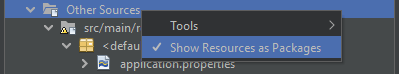
\includegraphics[scale=1]{imagens/cap10ShowResourcesAsPackages}
    \\\textbf{Fonte:} Elaborada pelo autor
    \label{fig:cap10ShowResourcesAsPackages}
\end{figure}
\FloatBarrier

Fazendo isso, a exibição dessa pasta se tornará a exibição padrão de árvore de diretórios, como mostrado na Figura\ref{fig:cap10EstruturaProjetoOK}. Dentro dela teremos inicialmente três itens: 1) O diretório \destaque{\texttt{static}} que usaremos para armazenar todos os arquivos que conterão conteúdo estático, como imagens e outros arquivos de mídia, arquivos CSS, arquivos JavaScript etc; 2) o diretório \destaque{\texttt{templates}} que conterá todos os \textit{templates} (modelos) que serão processados pelo \textit{framework} Thymeleaf e, 3) o arquivo \destaque{\texttt{application.properties}} que armazenará pares chave/valor, que serão utilizados pelo Spring Boot para alterar as configurações das dependências do projeto. Eu sei que já começaram a aparecer algumas coisas que ainda não foram explicadas, mas não se preocupe que logo veremos a serventia de cada uma delas.

\FloatBarrier
\begin{figure}[!htbp]
    \centering
    \caption{Estrutura do projeto}
    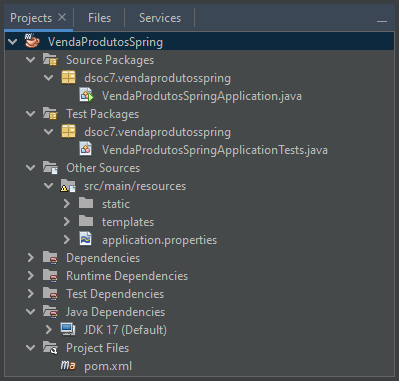
\includegraphics[scale=1]{imagens/cap10EstruturaProjetoOK}
    \\\textbf{Fonte:} Elaborada pelo autor
    \label{fig:cap10EstruturaProjetoOK}
\end{figure}
\FloatBarrier

Ainda sobre a estrutura do projeto, as pastas \destaque{\textit{Dependencies}}, \destaque{\textit{Runtime Dependencies}} e \destaque{\textit{Test Dependencies}} contém respectivamente as dependências de compilação, execução e teste do projeto. Os conteúdos delas não serão exibidos, pois contém muitos itens e eles são gerenciados diretamente pelo Maven. Na pasta \destaque{\textit{Java Dependencies}} é mostrado qual o JDK está em uso, no meu caso o 17, sendo que pode ser qualquer um com versão maior ou igual à 11 e, em \destaque{\textit{Project Files}} há um arquivo denominado \destaque{\texttt{pom.xml}} que contém as configurações do Maven para o nosso projeto. Eu não mostrarei o conteúdo aqui, pois ele estará disponível para vocês. Abra-o para dar uma olhada e siga o texto para entender o que está acontecendo em algumas de suas partes.

Entre as linhas 5 e 10 é informado que este projeto é do tipo Spring Boot, versão 2.6.2, lembrando que a versão pode variar. Entre as linhas 11 e 18 são mostrados os valores correspondentes aos metadados que preenchemos no Spring Initializr, com uma única adição, a tag \inlineHTMLCode{<version>} usada para informar a versão do projeto. Por padrão, a versão inicial vem com o conteúdo \texttt{0.0.1-SNAPSHOT}. Se você quiser mudar esse valor, fique à vontade! Agora, entre as linhas 19 e 58 são definidas todas as dependências que escolhemos no Spring Initializr. Se quisermos adicionar mais dependências, podemos editar diretamente esse arquivo ou ir no Spring Initializr, escolher a dependência que queremos inserir como gerenciada pelo Spring Boot, clicar no botão \destaque{\textit{EXPLORE}}, copiar o trecho de código XML e colar no nosso arquivo \destaque{\texttt{pom.xml}}. Dependências que não são gerenciadas pelo Spring Boot, como outras bibliotecas, também podem ser inseridas.


\subsection{Configurando e Executando a Aplicação}

Agora que já conhecemos a estrutura do projeto, poderíamos tentar executá-lo, mas como adicionamos várias dependências, nós vamos precisar configurar algumas primeiro, senão a execução não vai funcionar. Note que para colocar o projeto em execução nós \textbf{NÃO} usaremos o botão \textit{play} do NetBeans. Logo veremos como fazer. No momento vamos forçar na configuração, editando o arquivo \destaque{\texttt{application.properties}}. Abra-o e copie o conteúdo apresentado na Listagem~\thechapter.\ref{listagem:projetos/capitulo10/parciais/application01.properties}.

\propertiesCode{Primeira versão do arquivo de configuração do Spring Boot (\texttt{application.properties})}{projetos/capitulo10/parciais/application01.properties}

\begin{saibaMais}
    A lista completa das propriedades que podem ser configuradas no arquivo \texttt{application.properties} pode ser acessada a partir desse endereço: \url{https://docs.spring.io/spring-boot/docs/current/reference/html/application-properties.html}
\end{saibaMais}

Veja que todo o conteúdo está explicado com comentários, então não repetirei o que já foi explicado. Ainda atualizaremos esse arquivo algumas vezes durante a construção da nossa aplicação de exemplo. Vale ainda ressaltar que esse arquivo de configuração pode também ser escrito no formato YAML~\footnote{\textit{Yet Another Markup Language} \url{https://en.wikipedia.org/wiki/YAML}}. Por fim, antes de executarmos nosso projeto pela primeira vez, precisamos colocar o MariaDB no ar e criar o banco de dados com o nome de \destaque{\texttt{venda\_produtos\_spring}}. Faça isso.

Agora vamos executar nosso projeto! Logo abaixo da estrutura do projeto no NetBeans há a aba \destaque{\textit{Navigator}}. Quando o nó raiz do projeto estiver selecionado --na verdade alguns outros nós também-- serão apresentados todos os \textit{goals}/abjetivos/ações do Maven que estão disponíveis, sejam do próprio Maven ou através de \textit{plugins} definidos no arquivo \texttt{pom.xml}. Na Figura~\ref{fig:cap10PluginsMaven} essa aba é apresentada.

\FloatBarrier
\begin{figure}[!htbp]
    \centering
    \caption{\textit{Plugins} do Maven disponibilizados}
    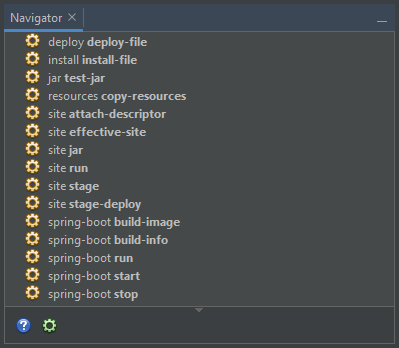
\includegraphics[scale=1]{imagens/cap10PluginsMaven}
    \\\textbf{Fonte:} Elaborada pelo autor
    \label{fig:cap10PluginsMaven}
\end{figure}
\FloatBarrier

Sendo assim, clique no nome do projeto para a aba \destaque{\textit{Navigator}} ser preenchida pelos \textit{goals} disponíveis. De todos eles, usaremos alguns. O usado para colocar o projeto no ar, compilando-o e iniciando o servidor é o \destaque{\texttt{spring-boot run}}. Clique duas vezes nele e você verá na tela de saída o Spring Boot iniciando o processo. Se tudo der certo, você terá como última linha da saída uma mensagem informando que a inicialização foi completada. Com isso, abra seu navegador (teremos que fazer isso manualmente) e acesse o endereço \url{http://localhost:8080/}. Uma página de erro será apresentada, haja vista que ainda não temos praticamente nada dentro do nosso projeto, mas com isso já sabemos que o servidor está no ar com o projeto.

Por falar em servidor, nos Capítulos anteriores tivemos que lidar com o GlassFish lembra-se? Como estamos usando o Spring MVC como dependência, o Spring Boot usará uma versão do Tomcat, que é um contêiner de Servlet como já aprendemos, embarcado no Spring MVC! Super legal não? Com isso não temos que nos preocupar com servidores durante o desenvolvimento da aplicação! Além disso, dependendo de onde a aplicação for ser implantada, poderemos executá-la igual faríamos com um \texttt{.jar} comum. Veremos isso posteriormente, além de tratarmos dos detalhes do empacotamento em arquivos \texttt{.war} para implantação em servidores remotos.

Vamos continuar, criando uma página inicial para o nosso projeto. Clique com o botão direito na pasta \destaque{\textit{templates}}, vá em \destaque{\textit{New}} e escolha \destaque{\textit{HTML File...}}. Se não houver essa opção, vá em \destaque{\textit{Other...}} e no diálogo que aparecerá, escolha a categoria \destaque{\textit{Other}}, provavelmente o último elemento da lista e do lado direito, no tipo de arquivo, \destaque{\textit{HTML File}}. Dê ok e siga o assistente, nomeando o arquivo como \destaque{\texttt{index}}. O conteúdo que seu arquivo HTML deve ter é o apresentado na Listagem~\thechapter.\ref{listagem:projetos/capitulo10/venda-produtos-spring/src/main/resources/templates/index.html}.

\htmlCode{Página inicial da aplicação (\texttt{/resources/templates/\\
index.html)}}{projetos/capitulo10/venda-produtos-spring/src/main/resources/templates/index.html}

Provavelmente seu projeto já está em execução, então volte ao navegador, ainda na URL \url{http://localhost:8080/} e atualize a página. Agora você verá uma página em branco com o conteúdo ``Sistema de Venda de Produtos Usando Spring Boot'' em destaque devido à \textit{tag} \inlineHTMLCode{<h1>}. Note que em comparação com o modelo usado pelo NetBeans para criar o \destaque{\texttt{index}}, a nossa versão possui algumas novidades, sendo assim, vamos explorá-las.

Perceba que a \textit{tag} \inlineHTMLCode{<html>} agora contém dois atributos. O primeiro, \inlineHTMLCode{xmlns} (XML \textit{Name Space}), indica ao navegador e também ao NetBeans --principalmente-- que nosso código HTML deve estar em conformidade com o formato \textit{EXtensible HyperText Markup Language} (XHTML), forçando que todas as nossas \textit{tags} estejam formatadas corretamente, de acordo com a versão 5 do HTML. Digo que isso é importante principalmente para o NetBeans, pois são essas duas modificações que guiarão o editor da ferramenta na acusação de erros. Para os navegadores também é importante, mas normalmente eles vão tentar se virar na hora que encontrarem erros no código HTML. O outro atributo, \inlineHTMLCode{xmlns:th}, indica que estamos criando um outro \textit{namespace}, chamado de \inlineHTMLCode{th} e associando o mesmo às \textit{tags} e atributos definidos pelo Thymeleaf. Poderia ser qualquer coisa ao invés de \inlineHTMLCode{th}, mas seguiremos o padrão. Veja que um paralelo que podemos fazer com algo que já vimos seria com as \textit{tags} da JSTL. Esse tal de Thymeleaf já apareceu algumas vezes no texto e ele logo será explicado, fique tranquilo! Note que agora precisamos obrigatoriamente terminar a \textit{tag} \inlineHTMLCode{<meta>} com uma barra, o que não era necessário se não houvesse essa restrição de conformidade ao XHTML.

Vamos fazer mais um teste para ver o que acontece. Acesse a URL \url{http://localhost:8080/index} ou \url{http://localhost:8080/index.html}. O que aconteceu? Erro novamente! Aí você se pergunta: ``Afinal, eu já não tenho o arquivo do index no projeto? Porque a URL não `funciona'?''. A resposta está em como o Spring MVC funciona. Todo e qualquer recurso que fará parte da camada \textit{View} precisa de alguma forma ser ``registrado'', associando um caminho relativo, que será exposto como URL, e o recurso em si. Automaticamente, a raiz do contexto é associada a um arquivo chamado \texttt{index.html}, mas se quisermos acessar esse arquivo de outra forma, precisamos dizer isso ao Spring MVC. Quando formos implementar nossos controladores e ao utilizar o Thymeleaf, esses registros serão feitos programaticamente, seja nas classes dos controladores, por meio de anotações, ou no código dos \textit{templates}, mas se quisermos que outro recurso seja exposto, precisamos informar isso ao \textit{framework}. Vamos fazer isso? Note que o que vamos fazer é totalmente opcional no nosso caso, mas faremos para termos como exemplo e caso você precise realizar tal operação.


\subsection{Realizando Configurações Programaticamente}

A primeira coisa que faremos é criar um novo pacote, chamado de \destaque{\texttt{web}}, dentro do pacote \destaque{\texttt{dsoc7.vendaprodutosspring}}. Cuidado, estamos trabalhando nos pacotes de código fonte, não nos pacotes de teste! Outra coisa importante. Todo e qualquer código que será gerenciado pelo Spring Boot, pelo Spring Framework e pelo Spring MVC precisa estar, obrigatoriamente, dentro do pacote principal do projeto, no nosso caso o pacote \destaque{\texttt{dsoc7.vendaprodutosspring}} que contém a classe \destaque{\texttt{VendaProdutosSpringApplication}} ou em subpacotes do mesmo.

No pacote \destaque{\texttt{dsoc7.vendaprodutosspring.web}} recém criado, crie uma classe chamada de \inlineJavaCode{WebConfig}. O nome poderia ser qualquer coisa, mas vamos chamar assim para darmos a noção que essa classe fará a configuração da parte ``web'' do Spring MVC. Veja o código da classe na Listagem~\thechapter.\ref{listagem:projetos/capitulo10/venda-produtos-spring/src/main/java/dsoc7/vendaprodutosspring/web/WebConfig.java}.

\javaCode{Classe de configuração\\
(\texttt{dsoc7/vendaprodutosspring/web/WebConfig.java)}}{projetos/capitulo10/venda-produtos-spring/src/main/java/dsoc7/vendaprodutosspring/web/WebConfig.java}

Na linha 12 usamos uma anotação \inlineJavaCode{@Configuration} do Spring Framework, que informa ao Spring que essa classe é uma classe de configuração, ou seja, ela executará tarefas de configuração da aplicação. Essa classe implementa a interface \inlineJavaCode{WebMcvConfigurer}, que define vários métodos para configurar programaticamente o Spring MVC. O método que vamos implementar no momento é o \inlineJavaCode{addViewControllers}, que pelo nome podemos perceber que irá realizar a adição de controladores de visualizações na nossa aplicação. Esse método tem como parâmetro um \inlineJavaCode{ViewControllerRegistry} que é o tal do registro que associa um caminho à um recurso --normalmente uma \textit{view}-- e que será usado pelo Spring MVC para chegar até o recurso desejado pela URL requisitada. No nosso exemplo, adicionamos dois caminhos ao recurso \destaque{\texttt{index}}. Na linha 18, o primeiro caminho, \destaque{\texttt{/index}}, é associado ao recurso \destaque{\texttt{index}} e o caminho \destaque{\texttt{/index.html}} é associado ao mesmo recurso. Note que o caminho parte da raiz da aplicação e que o recurso está contido na pasta \destaque{\texttt{templates}} do projeto. Salve sua classe se ainda não o fez e vá no navegador testar as duas URLs que não estavam funcionando. O que aconteceu? Agora sim não é?


\subsection{O Ponto de Entrada de Uma Aplicação Spring Boot}

Vamos continuar a explorar essa fase inicial de preparação e de entendimento do nosso projeto? Uma aplicação Spring Boot pode ser tanto Web como Desktop. A nossa é Web, óbvio. Enquanto em aplicações Web ``tradicionais'' não existe muito bem definido um ponto de entrada da execução da aplicação (um ``método \texttt{main}''), pois isso fica escondido atrás dos servidores de aplicação e dos dos contêineres de Servlets, numa aplicação Spring Boot isso é definido. Veja que dentro do pacote \destaque{\texttt{dsoc7.vendaprodutosspring}} há uma classe, que já mencionamos a alguns parágrafos, chamada de \inlineJavaCode{VendaProdutosSpringApplication}, criada automaticamente pelo Spring Initializr. O código da mesma pode ser visto na Listagem~\thechapter.\ref{listagem:projetos/capitulo10/venda-produtos-spring/src/main/java/dsoc7/vendaprodutosspring/VendaProdutosSpringApplication.java}.

\javaCode{Classe de definição de aplicação Spring Boot\\
(\texttt{dsoc7/vendaprodutosspring/VendaProdutosSpringApplication.java)}}{projetos/capitulo10/venda-produtos-spring/src/main/java/dsoc7/vendaprodutosspring/VendaProdutosSpringApplication.java}

Essa classe está anotada com \inlineJavaCode{@SpringBootApplication}, que é uma anotação do Spring Boot e que indica que essa classe é uma aplicação Spring Boot. Essa classe deve ter um método \texttt{main}, normalmente com uma linha de código e, apesar de poder haver configurações implementadas nela, deixaremos isso para as classes de configuração como a \inlineJavaCode{WebConfig} que criamos há pouco. Na linha de código presente dentro do método \texttt{main} o método estático \texttt{run} da classe \inlineJavaCode{SpringApplication} é executado, passando-se uma referência ao tipo da classe \inlineJavaCode{VendaProdutosSpringApplication} e os argumentos que porventura foram fornecidos ao método \texttt{main}. Não precisaremos mexer com ela se formos trabalhar com empacotamento em \texttt{.jar}, mas se mudarmos para \texttt{.war} precisaremos fazer algumas modificações. Isso fica para depois, como já falei.


\subsection{Atualizações Automáticas do Navegador Usando LiveReload}

Estamos quase terminando essa parte introdutória! Vamos tratar agora sobre outra funcionalidade que nos ajuda na produtividade. Toda vez que alteramos algo no projeto, já sabemos que o Spring Boot DevTools vai atualizar os arquivos do projeto no Tomcat que está em execução, bastando irmos no navegador e atualizar a página para testarmos o que acabamos de fazer. Isso já nos poupa de mandar o projeto rodar de novo em algumas situações. Agora vamos ver o que podemos fazer para a atualização da página ser automática, ou seja, ao alterarmos algo no projeto e salvarmos, a página já estará atualizada ou em processo de atualização no navegador.

Para isso, precisamos instalar uma extensão no Chrome (\url{http://livereload.com/}), chamada de \destaque{LiveReload}. Há versões para outros navegadores também, mas detalharei a versão do Chrome, pois é o navegador que eu uso e que provavelmente a maioria de vocês também. Para a instalação no Chrome, entre na seção de extensões da Chrome Web Store (\url{https://chrome.google.com/webstore/category/extensions}) e na caixa de pesquisa, procure por LiveReload. Pode ser que haja mais de um resultado. A que estamos procurando é a ``oferecida por \url{http://livereload.com/}'' e versão atual é a 2.1.0, mas isso, como você já sabe, pode variar de acordo com a época que você está lendo este livro. Clique nela e depois no botão \destaque{Usar no Chrome}. Isso fará com que um botão\footnote{Algo parecido com isso 
\includegraphics[scale=1]{imagens/cap10BotaoLiveReloadBranco}, ou isso 
\includegraphics[scale=1]{imagens/cap10BotaoLiveReloadPreto}.} seja adicionado na barra de endereços do Chrome. Ao clicar nele uma vez, o LiveReload será ativado. A partir de agora, toda alteração que for feita em arquivos HTML, CSS, JavaScript etc, disparará uma atualização automática na página que está atualmente sendo mostrada, visto que o DevTools enviará, via WebSocket, uma notificação ao LiveReload. Faça um teste. Mude algo no \texttt{index.html}, salve e volte ao navegador. A alteração ou já estará sendo exibida ou a página estará sendo atualizada. Se ainda não estiver funcionando matando o \textit{goal} \destaque{\texttt{spring-boot run}} que ainda está em execução clicando no \texttt{x} do indicador de processos do NetBeans\footnote{Canto inferior direito, algo parecido com isso 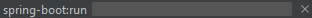
\includegraphics[scale=1]{imagens/cap10MatarProcessoSpringBootRun}}, a inicie novamente com o \textit{goal} \destaque{\texttt{spring-boot run}}, atualize a página no Chrome, faça a alteração no código HTML do \texttt{index.html} e veja a atualização ser feita automaticamente a partir de agora. Deve funcionar.

Muito bem! Temos a infraestrutura básica do nosso projeto pronta para podermos começar a trabalhar de verdade! Iremos agora começar a construir novamente, camada por camada, nossa aplicação de Venda de Produtos, mas agora usando diversas bibliotecas, \textit{frameworks} e recursos que, graças ao Spring Boot, já estão prontos para serem utilizados. Para não ficar muito extenso e cansativo, irei focar em algumas entidades para você aprender o que quero ensinar. O código completo do projeto estará disponível para consulta, como de praxe. Vamos lá!


\section{Hibernate, JPA, Validações e Lombok}

criação das entidades

netbeans vai reclamar que o projeto não tem undidade de persistência (resolução via IOC do Spring)

carga inicial no banco através do import.sql


\section{Spring MVC}

criação dos controladores e páginas com thymeleaf

importância das diretivas de pré-processamento, de busca de propriedades, de resolução de contexto etc.

\begin{comment}
    @{}, ${}, *{}, __${}__, T(classe).métodoEstático, tags th, blocos sintáticos
\end{comment}


\subsection{Outros \textit{Frameworks} MVC}

%Falar brevemente de: JavaServer Faces (JSF), Struts, VRaptor etc.

\section{Execução Local do Projeto}

falar do .jar


\section{Resumo}

\section{Exercícios}

\section{Projetos}
